\section{U-Net Family}

The first model family implemented in this project is U-Net~\cite{DBLP:conf/miccai/RonnebergerFB15}. In this work, U-Net is used as a configurable encoder-decoder architecture for paired low-light image enhancement. This choice naturally matches the image-to-image nature of the task: the model receives a low-light RGB image and must produce an enhanced RGB image at the corresponding spatial resolution. Although U-Net was originally introduced for biomedical image segmentation, its encoder-decoder structure with skip connections is also well suited to this setting, because it allows the model to combine global contextual information with the preservation of local image details. The corresponding grid search explores multiple configurations by varying both architectural and optimization choices.

\subsection{Architecture}

U-Net is an encoder-decoder architecture with skip connections. The encoder progressively reduces the spatial resolution of the image and extracts increasingly abstract features, while the decoder restores the spatial resolution and produces the enhanced RGB image. The deepest part of the network is called the bottleneck: it is the point where the feature maps have the lowest spatial resolution but the richest semantic representation. Skip connections transfer encoder features to decoder stages at matching resolutions, except at this bottleneck level, where no skip connection is needed. This helps the decoder recover spatial details that may be weakened during downsampling, while still using the contextual information extracted by the deeper layers.

The implemented U-Net is built from repeated convolutional blocks. A convolutional layer learns local filters over the image or over intermediate feature maps. A feature map is an internal representation produced by the network: it can be seen as a set of channels that store the patterns detected at a given layer, such as edges, textures, colors, or more abstract structures. In this implementation, each block applies two convolutional layers, and each convolution is followed by two possible operations: normalization, when enabled, and a non-linear activation function.

In each convolutional block, the convolutions use a $3 \times 3$ kernel with padding equal to one. This choice preserves the spatial resolution inside the block, so that feature maps are not progressively reduced by the convolutions themselves. Spatial resolution changes are therefore confined to the explicit downsampling and upsampling stages. This is useful for paired image enhancement, where preserving spatial correspondence between the prediction and the reference target is important for pixel-wise supervision.

The normalization layer is optional, and different normalization strategies are part of the search space. Normalization can make training more stable by controlling the distribution of intermediate feature values. The activation function is instead kept fixed to leaky rectified linear unit (LeakyReLU) in the U-Net experiments. A ReLU-family activation is appropriate for this image-enhancement setting because it is simple, efficient, and piecewise linear, which helps convolutional features preserve local contrast, edges, and texture responses without compressing them through saturating hidden activations. This is useful in low-light enhancement, where weak structures in dark regions must remain available to the decoder instead of being overly smoothed or suppressed. LeakyReLU is used as a slightly more robust ReLU variant: instead of setting all negative activations exactly to zero, it keeps a small non-zero response for them. This reduces the risk of discarding weak intermediate signals and helps maintain gradient flow during training.

Downsampling is performed with $2 \times 2$ max pooling followed by a convolutional block. Max pooling reduces the spatial size of the feature maps, allowing deeper layers to process a larger image context. Upsampling is performed either with bilinear interpolation or with transposed convolution, depending on the configuration. Bilinear interpolation is a fixed, non-learnable resizing operation. Transposed convolution is instead learnable, so the model can adapt how feature maps are upsampled.

The final layer is a $1 \times 1$ convolution followed by a sigmoid function. The $1 \times 1$ convolution maps the decoder features to the three RGB output channels. The sigmoid function constrains the output values to the $[0,1]$ range, matching the normalized image representation used throughout the pipeline.

\subsection{Training Objective and Grid Search}

The U-Net family follows the general experimental protocol described in Section~\ref{sec:experimental_protocol}. For this family, training uses a combined L1-SSIM objective. The L1 term penalizes pixel-wise differences between the enhanced output and the reference image, using the MAE defined in Eq.~\ref{eq:mae}. The structural term is implemented as an SSIM-based penalty, using the SSIM definition in Eq.~\ref{eq:ssim}. Since SSIM is a similarity score to maximize, it is converted into a loss term by using $1 - \mathrm{SSIM}$, which becomes smaller when the prediction is structurally closer to the reference image. The loss is defined as
\begin{equation}
	\mathcal{L}(\hat{I}, I)
	=
	0.8 \, \mathrm{MAE}(\hat{I}, I)
	+
	0.2 \, \bigl(1 - \mathrm{SSIM}(\hat{I}, I)\bigr),
	\label{eq:l1_ssim_loss}
\end{equation}
where $\hat{I}$ is the enhanced output and $I$ is the reference image. The two coefficients are configurable in the experiment file, but they are kept fixed in the grid search.

The grid search defined for this family explores a set of architectural and optimization choices. The architectural part of the grid varies the channel schedule, the normalization strategy, and the upsampling method. The channel schedule specifies how many feature channels are used at each resolution level of the U-Net. As the encoder goes deeper, the spatial resolution decreases and the number of channels usually increases, allowing the network to represent progressively richer features. Therefore, a smaller channel schedule defines a lighter model with fewer parameters, while a larger schedule increases model capacity at the cost of higher computational complexity. The explored hyperparameter space is:

\begin{itemize}[topsep=5pt]
	\item Channel schedule $\in$ $(16,32,64,128)$, $(32,64,128,256)$, $(32,64,128,256,512)$;
	\item Normalization $\in$ none, batch, instance, group;
	\item Upsampling $\in$ bilinear interpolation, transposed convolution;
	\item Learning rate $\in$ $3{\cdot}10^{-4}$, $5{\cdot}10^{-4}$, $10^{-3}$;
	\item Weight decay $\in$ $0$, $10^{-4}$.
\end{itemize}

The normalization choice determines how intermediate feature activations are normalized inside the convolutional blocks. The search compares no normalization, batch normalization, instance normalization, and group normalization. These alternatives differ in the statistics used for normalization, respectively relying on mini-batch statistics, per-image statistics, or groups of channels. For group normalization, the number of groups is fixed and is not part of the grid.

The upsampling method controls how decoder feature maps are brought back to higher spatial resolutions. Transposed convolution is a learnable upsampling operation and represents a standard choice in encoder-decoder architectures. However, as discussed by Odena et al. in \emph{Deconvolution and Checkerboard Artifacts}~\cite{odena2016deconvolution}, learned upsampling operators such as transposed convolutions may introduce visible periodic artifacts when not properly controlled. For this reason, the grid also includes bilinear interpolation, which performs a fixed non-learnable resize before the following convolutional block. This alternative is less flexible, but provides a simpler upsampling mechanism and can reduce the risk of upsampling artifacts.

Finally, the grid varies two optimization hyperparameters: the learning rate and the weight decay. The learning rate controls the magnitude of the optimizer updates, while weight decay acts as a regularization term on the model weights.

Combining these choices gives 144 U-Net configurations in the single-seed screening stage.

\subsection{Quantitative Analysis}

This subsection reports the quantitative behavior of the selected U-Net family. The final configuration is the one selected by the fixed experimental protocol of this project, and has $7.76$M trainable parameters. Table~\ref{tab:unet_final_evaluation} reports the final evaluation of the selected U-Net configuration.

\begin{table*}[t]
	\centering
	\caption{Final evaluation of the selected U-Net configuration. The first row reports the held-out in-domain evaluation, the following three rows report independent external evaluation results, and LOL-v1 (overlap) is reported for descriptive transparency only and is excluded from independent cross-dataset conclusions. Values are reported as mean $\pm$ standard deviation across three seeds. Full-reference metrics are not available for ExDark because it is unpaired.}
	\label{tab:unet_final_evaluation}
	\resizebox{\textwidth}{!}{
		\begin{tabular}{lccccccccccc}
			\toprule
			Dataset & SSIM & PSNR (dB) & MAE & NIQE & BRISQUE & Mean $Y$ & Std $Y$ & Dark (\%) & Clip (\%) & RGBI & Lap. sharp. \\
			\midrule
			LOL-v2 Real & $0.849 \pm 0.003$ & $19.54 \pm 0.37$ & $0.105 \pm 0.003$ & $6.55 \pm 0.47$ & $27.30 \pm 2.20$ & $0.459 \pm 0.004$ & $0.160 \pm 0.008$ & $1.3 \pm 0.5$ & $0.07 \pm 0.01$ & $0.039 \pm 0.004$ & $0.0088 \pm 0.0006$ \\
			\midrule
			LOL-v2 Synthetic & $0.766 \pm 0.006$ & $17.14 \pm 0.08$ & $0.129 \pm 0.001$ & $6.92 \pm 0.20$ & $31.75 \pm 1.41$ & $0.446 \pm 0.009$ & $0.212 \pm 0.010$ & $3.5 \pm 2.1$ & $0.11 \pm 0.04$ & $0.032 \pm 0.002$ & $0.0090 \pm 0.0006$ \\
			MILLs & $0.755 \pm 0.005$ & $17.17 \pm 0.15$ & $0.132 \pm 0.004$ & $6.16 \pm 0.13$ & $23.22 \pm 1.36$ & $0.454 \pm 0.022$ & $0.119 \pm 0.002$ & $0.9 \pm 0.3$ & $0.00 \pm 0.00$ & $0.074 \pm 0.004$ & $0.0056 \pm 0.0006$ \\
			ExDark & -- & -- & -- & $6.89 \pm 0.29$ & $33.37 \pm 1.30$ & $0.407 \pm 0.005$ & $0.195 \pm 0.009$ & $5.1 \pm 2.2$ & $0.12 \pm 0.04$ & $0.070 \pm 0.001$ & $0.0074 \pm 0.0004$ \\
			\midrule
			LOL-v1 (overlap) & $0.884 \pm 0.003$ & $22.10 \pm 0.31$ & $0.077 \pm 0.003$ & $6.77 \pm 0.31$ & $28.75 \pm 2.00$ & $0.468 \pm 0.005$ & $0.177 \pm 0.007$ & $2.7 \pm 0.7$ & $0.05 \pm 0.01$ & $0.047 \pm 0.003$ & $0.0084 \pm 0.0005$ \\
			\bottomrule
		\end{tabular}
	}
\end{table*}

\analysispar{In-domain and cross-dataset evaluation}
LOL-v2 Real is the in-domain reference, because it comes from the same dataset and acquisition setting used for training and validation.

The independent paired external datasets show a clearer domain shift. LOL-v2 Synthetic and MILLs both have lower full-reference quality than LOL-v2 Real, with SSIM around $0.76$ and MAE around $0.13$. This is important because LOL-v2 Synthetic still belongs to the LOL-v2 family, but its synthetic degradation process differs from the real low-light acquisition used for training. MILLs confirms the same limitation under a different paired dataset. Therefore, the selected U-Net provides strong in-domain reconstruction, but its reconstruction quality decreases when the low-light formation process changes.

The no-reference metrics should be read as complementary indicators. MILLs obtains the best BRISQUE value among the independent paired external datasets, even though its SSIM, PSNR, and MAE are worse than those of LOL-v2 Real. This shows that no-reference naturalness scores do not necessarily measure closeness to the paired target. For paired datasets, SSIM, PSNR, and MAE remain the most direct evidence of reconstruction quality, while NIQE and BRISQUE are mainly useful to support the interpretation of perceptual quality and to evaluate unpaired data.

Diagnostic metrics show how the model changes brightness and contrast. Across LOL-v2 Real, LOL-v2 Synthetic, and MILLs, mean output luminance stays within $0.446$--$0.459$, suggesting that the U-Net maps them to a similar brightness level. ExDark differs, with the lowest mean luminance ($0.407$) and highest dark-pixel ratio ($5.1\%$). Although it brightens these unpaired real-world dark images, which lie outside the LOL-v2 Real distribution, it leaves more regions under-exposed. RGB imbalance is also higher on MILLs and ExDark than on LOL-v2 Real, indicating greater cross-dataset color-shift risk.

Finally, LOL-v1 is reported only as an overlap-control result. Because LOL-v1 low-light inputs overlap with LOL-v2 Real images across its train, validation, and test partitions, they are not interpreted as independent transfer evidence.

\analysispar{MILLs illumination-level analysis}
MILLs is paired, and its illumination-level metadata makes it possible to analyze how the U-Net behaves as input brightness changes. Table~\ref{tab:unet_mills_illumination} reports the results grouped by illumination level.

\begin{table*}[t]
	\centering
	\caption{MILLs illumination-level results for the selected U-Net configuration. Values are reported as mean $\pm$ standard deviation across three seeds. MILLs is paired, so full-reference, no-reference, and diagnostic metrics are reported. Bold values mark the best score for each full-reference and no-reference metric.}
	\label{tab:unet_mills_illumination}
	\resizebox{\textwidth}{!}{
		\begin{tabular}{cccccccccccc}
			\toprule
			Level & SSIM & PSNR (dB) & MAE & NIQE & BRISQUE & Mean $Y$ & Std $Y$ & Dark (\%) & Clip (\%) & RGBI & Lap. sharp. \\
			\midrule
			1 & $0.698 \pm 0.002$ & $17.22 \pm 0.43$ & $\mathbf{0.119 \pm 0.006}$ & $6.26 \pm 0.43$ & $\mathbf{22.66 \pm 1.99}$ & $0.435 \pm 0.015$ & $0.167 \pm 0.006$ & $3.3 \pm 2.1$ & $0.00 \pm 0.00$ & $0.077 \pm 0.008$ & $0.0073 \pm 0.0006$ \\
			2 & $0.739 \pm 0.008$ & $16.62 \pm 0.22$ & $0.140 \pm 0.004$ & $\mathbf{6.11 \pm 0.18}$ & $23.96 \pm 1.75$ & $0.467 \pm 0.016$ & $0.128 \pm 0.003$ & $1.5 \pm 0.6$ & $0.00 \pm 0.00$ & $0.080 \pm 0.003$ & $0.0060 \pm 0.0005$ \\
			3 & $0.753 \pm 0.007$ & $16.87 \pm 0.12$ & $0.138 \pm 0.004$ & $6.14 \pm 0.16$ & $23.30 \pm 1.45$ & $0.463 \pm 0.020$ & $0.119 \pm 0.002$ & $1.1 \pm 0.3$ & $0.00 \pm 0.00$ & $0.076 \pm 0.004$ & $0.0056 \pm 0.0005$ \\
			4 & $0.758 \pm 0.006$ & $17.01 \pm 0.13$ & $0.136 \pm 0.004$ & $6.13 \pm 0.15$ & $23.37 \pm 1.28$ & $0.460 \pm 0.022$ & $0.115 \pm 0.001$ & $0.8 \pm 0.2$ & $0.00 \pm 0.00$ & $0.075 \pm 0.004$ & $0.0054 \pm 0.0006$ \\
			5 & $0.762 \pm 0.006$ & $17.15 \pm 0.15$ & $0.133 \pm 0.004$ & $6.16 \pm 0.13$ & $23.16 \pm 1.21$ & $0.456 \pm 0.023$ & $0.113 \pm 0.001$ & $0.6 \pm 0.2$ & $0.00 \pm 0.00$ & $0.073 \pm 0.004$ & $0.0053 \pm 0.0006$ \\
			6 & $0.765 \pm 0.005$ & $17.26 \pm 0.16$ & $0.132 \pm 0.004$ & $6.16 \pm 0.12$ & $23.16 \pm 1.23$ & $0.454 \pm 0.024$ & $0.111 \pm 0.001$ & $0.5 \pm 0.2$ & $0.00 \pm 0.00$ & $0.073 \pm 0.004$ & $0.0053 \pm 0.0006$ \\
			7 & $0.766 \pm 0.005$ & $17.31 \pm 0.19$ & $0.131 \pm 0.005$ & $6.13 \pm 0.12$ & $23.08 \pm 1.23$ & $0.452 \pm 0.025$ & $0.110 \pm 0.001$ & $0.4 \pm 0.2$ & $0.00 \pm 0.00$ & $0.072 \pm 0.004$ & $0.0052 \pm 0.0006$ \\
			8 & $0.768 \pm 0.005$ & $17.36 \pm 0.22$ & $0.130 \pm 0.005$ & $6.18 \pm 0.15$ & $23.12 \pm 1.26$ & $0.451 \pm 0.025$ & $0.110 \pm 0.001$ & $0.4 \pm 0.2$ & $0.00 \pm 0.00$ & $0.071 \pm 0.005$ & $0.0052 \pm 0.0006$ \\
			9 & $\mathbf{0.770 \pm 0.005}$ & $\mathbf{17.47 \pm 0.25}$ & $0.128 \pm 0.006$ & $6.18 \pm 0.14$ & $23.14 \pm 1.22$ & $0.451 \pm 0.026$ & $0.109 \pm 0.001$ & $0.3 \pm 0.2$ & $0.00 \pm 0.00$ & $0.072 \pm 0.004$ & $0.0051 \pm 0.0006$ \\
			10 & $0.769 \pm 0.005$ & $17.43 \pm 0.26$ & $0.129 \pm 0.006$ & $6.19 \pm 0.13$ & $23.24 \pm 1.19$ & $0.449 \pm 0.026$ & $0.109 \pm 0.001$ & $0.3 \pm 0.2$ & $0.00 \pm 0.00$ & $0.070 \pm 0.005$ & $0.0051 \pm 0.0006$ \\
			\bottomrule
		\end{tabular}
	}
\end{table*}

The MILLs results show that the darkest illumination level is the most difficult one. Level 1 has the lowest SSIM, $0.698$, and the highest dark-pixel ratio, $3.3\%$. From level 2 onward, SSIM increases and reaches its maximum at level 9, while the dark-pixel ratio progressively decreases to about $0.3\%$ at the brightest levels. This indicates that the model preserves structure better when the input is less severely under-exposed.

PSNR and MAE do not follow a perfectly monotonic trend, especially at the first two illumination levels. This suggests that the errors are not only caused by average pixel differences, but also by structural and contrast-related changes. The diagnostic metrics support this interpretation: mean luminance remains within a limited interval, while the dark-pixel ratio decreases strongly across levels. In other words, the U-Net tends to enhance MILLs images toward a relatively stable brightness range, but its ability to recover structure is weaker when the starting illumination is very low.

\analysispar{ExDark category-level analysis}
ExDark is further analyzed by object category because it is unpaired and category metadata is available. Table~\ref{tab:unet_exdark_category} reports the category-level no-reference and diagnostic results.

\begin{table*}[t]
	\centering
	\caption{ExDark category-level results for the selected U-Net configuration. Values are reported as mean $\pm$ standard deviation across three seeds. ExDark is unpaired, so only no-reference and diagnostic metrics are reported. Bold values mark the best score for each no-reference metric.}
	\label{tab:unet_exdark_category}
	\resizebox{\textwidth}{!}{
		\begin{tabular}{lcccccccc}
			\toprule
			Category & NIQE & BRISQUE & Mean $Y$ & Std $Y$ & Dark (\%) & Clip (\%) & RGBI & Lap. sharp. \\
			\midrule
			Bicycle & $6.42 \pm 0.30$ & $31.34 \pm 1.61$ & $0.414 \pm 0.006$ & $0.191 \pm 0.009$ & $3.9 \pm 1.9$ & $0.09 \pm 0.03$ & $0.073 \pm 0.001$ & $0.0091 \pm 0.0007$ \\
			Boat & $7.71 \pm 0.28$ & $35.05 \pm 1.39$ & $0.422 \pm 0.000$ & $0.191 \pm 0.008$ & $4.9 \pm 1.4$ & $0.04 \pm 0.02$ & $0.069 \pm 0.003$ & $0.0075 \pm 0.0005$ \\
			Bottle & $6.75 \pm 0.26$ & $33.99 \pm 1.15$ & $0.388 \pm 0.008$ & $0.196 \pm 0.010$ & $7.4 \pm 2.6$ & $0.14 \pm 0.05$ & $0.080 \pm 0.001$ & $0.0066 \pm 0.0003$ \\
			Bus & $6.46 \pm 0.31$ & $34.71 \pm 1.43$ & $0.396 \pm 0.008$ & $0.191 \pm 0.010$ & $4.7 \pm 2.4$ & $0.11 \pm 0.03$ & $0.076 \pm 0.001$ & $0.0085 \pm 0.0006$ \\
			Car & $6.91 \pm 0.31$ & $34.04 \pm 1.42$ & $0.398 \pm 0.005$ & $0.192 \pm 0.010$ & $5.6 \pm 2.3$ & $0.18 \pm 0.07$ & $0.075 \pm 0.002$ & $0.0068 \pm 0.0004$ \\
			Cat & $6.82 \pm 0.27$ & $31.65 \pm 1.33$ & $0.418 \pm 0.004$ & $0.195 \pm 0.009$ & $4.5 \pm 2.2$ & $0.11 \pm 0.04$ & $0.066 \pm 0.002$ & $0.0066 \pm 0.0003$ \\
			Chair & $7.24 \pm 0.27$ & $34.56 \pm 1.24$ & $0.412 \pm 0.007$ & $0.201 \pm 0.010$ & $4.6 \pm 2.3$ & $0.14 \pm 0.05$ & $0.063 \pm 0.001$ & $0.0075 \pm 0.0004$ \\
			Cup & $7.57 \pm 0.31$ & $36.66 \pm 0.64$ & $0.389 \pm 0.010$ & $0.203 \pm 0.010$ & $7.4 \pm 3.0$ & $0.11 \pm 0.05$ & $0.077 \pm 0.001$ & $0.0060 \pm 0.0002$ \\
			Dog & $6.70 \pm 0.29$ & $\mathbf{31.28 \pm 1.30}$ & $0.423 \pm 0.004$ & $0.195 \pm 0.009$ & $4.2 \pm 1.8$ & $0.12 \pm 0.04$ & $0.066 \pm 0.001$ & $0.0068 \pm 0.0003$ \\
			Motorbike & $\mathbf{6.17 \pm 0.30}$ & $31.49 \pm 1.63$ & $0.409 \pm 0.006$ & $0.192 \pm 0.009$ & $4.5 \pm 2.0$ & $0.10 \pm 0.04$ & $0.073 \pm 0.001$ & $0.0085 \pm 0.0006$ \\
			People & $7.00 \pm 0.36$ & $32.45 \pm 1.33$ & $0.395 \pm 0.005$ & $0.193 \pm 0.009$ & $5.6 \pm 2.6$ & $0.14 \pm 0.05$ & $0.064 \pm 0.001$ & $0.0074 \pm 0.0004$ \\
			Table & $6.80 \pm 0.29$ & $34.74 \pm 1.22$ & $0.408 \pm 0.006$ & $0.200 \pm 0.010$ & $4.9 \pm 2.6$ & $0.12 \pm 0.05$ & $0.063 \pm 0.001$ & $0.0076 \pm 0.0003$ \\
			\bottomrule
		\end{tabular}
	}
\end{table*}

The ExDark category-level results show that performance is not uniform across scene types. According to NIQE, motorbike is the best category, while boat is the worst. According to BRISQUE, dog obtains the best score, while cup is the worst. Since both metrics are no-reference, these differences should not be interpreted as reconstruction errors with respect to a target. They indicate instead that some categories produce outputs that are closer to, or farther from, the natural-image statistics measured by these quality estimators.

The diagnostic metrics make the category differences easier to interpret. Bottle and cup have the lowest mean luminance, around $0.388$--$0.389$, and also the highest dark-pixel ratio, around $7.4\%$. These categories therefore remain the most under-exposed after enhancement. Car has the highest clipping ratio, suggesting that reflective surfaces or vehicle lights can produce localized over-bright regions. Bottle also has the largest RGB imbalance, which indicates a stronger risk of color cast. These results suggest that the ExDark behavior depends not only on the semantic category, but also on correlated visual properties such as object size, background darkness, reflective materials, and local light sources.

\analysispar{Summary}
Overall, the quantitative analysis shows a clear difference between in-domain and cross-dataset behavior. The selected U-Net is effective on the held-out LOL-v2 Real test set, but its full-reference performance drops on the independent external datasets LOL-v2 Synthetic and MILLs. ExDark further shows that, in an unpaired real-world setting, the model improves visibility but leaves more residual darkness and stronger diagnostic signs of domain shift. This confirms that the baseline U-Net learns a useful enhancement mapping, but does not fully generalize to all low-light distributions.

\subsection{Qualitative Analysis}

Visual inspection is useful to understand how the selected U-Net behaves beyond the average metric values. In particular, it shows whether the model only increases brightness, or whether it also preserves color, texture, edges, and realistic image content. Figure~\ref{fig:unet_qualitative} reports one successful enhancement example and a set of representative failure cases.

\begin{figure*}[p]
	\centering
	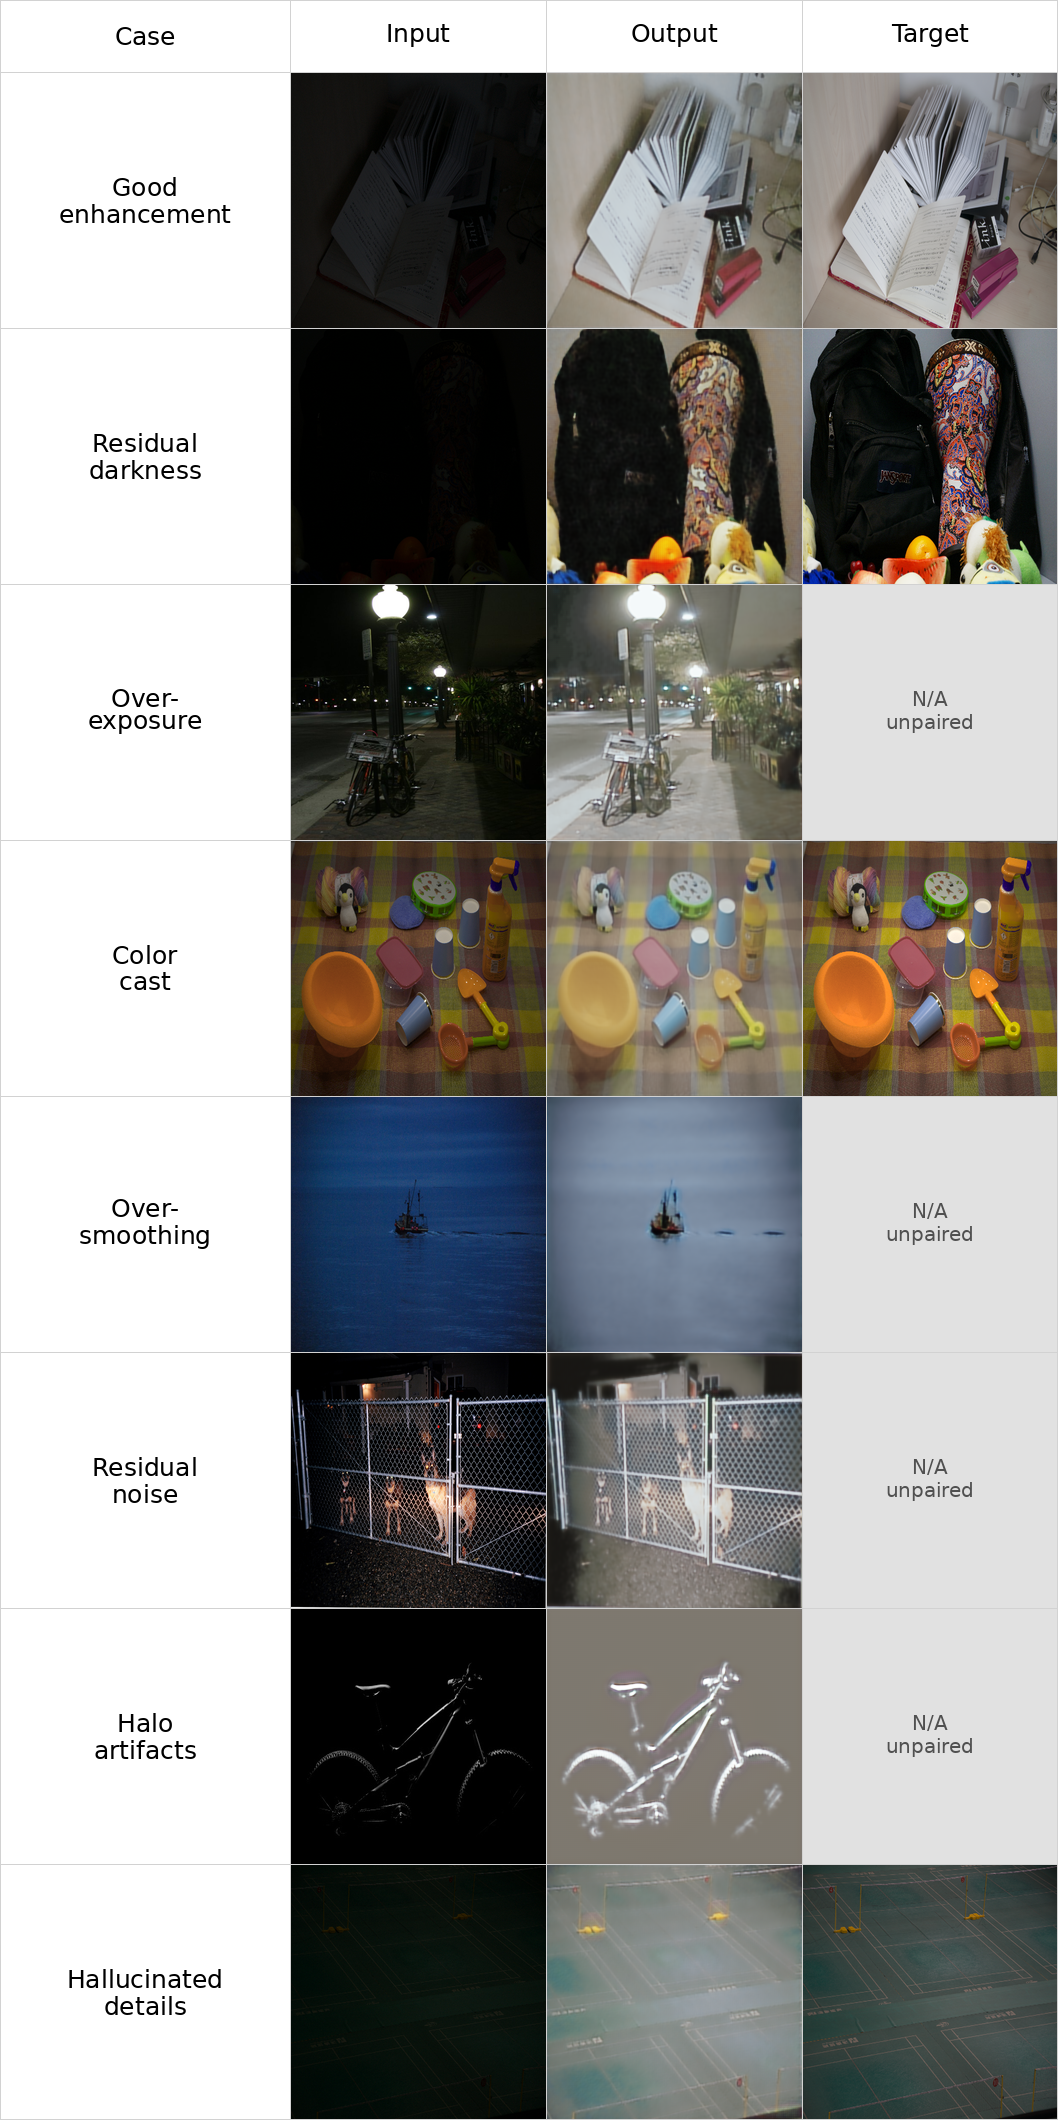
\includegraphics[
	height=\dimexpr\textheight-3\baselineskip\relax,
	keepaspectratio
	]{fig/unet_qualitative/unet_qualitative.png}
	\caption{Qualitative examples obtained with the selected U-Net configuration on different datasets used in the project. Each row shows the input, the enhanced output, and the target when available. The rows include one successful enhancement case and representative failure modes: residual darkness, over-exposure, color cast, over-smoothing, residual noise, halo artifacts, and hallucinated details.}
	\label{fig:unet_qualitative}
\end{figure*}

\analysispar{Hallucinated details}
The hallucinated details example was selected from LOL-v2 Real because the paired target makes the non-faithful structure easy to identify. The enhanced image contains a hazy diagonal pattern over the court, while the target remains cleaner and more uniform. This is a severe failure because the model is not only changing brightness or color, but also adding visual content that does not correspond to the reference. In a paired enhancement task, this behavior is especially problematic because the output should improve visibility without changing the underlying scene content. A possible reason is that the network tries to infer missing information from extremely weak input evidence. When the low-light input does not provide enough reliable detail, the model may produce plausible-looking local patterns that reduce training loss on average but are not faithful to the true scene.

\analysispar{Color cast}
The color-cast example was selected from MILLs because the paired target makes the chromatic error visible. The output is brighter than the input but introduces a yellow-green cast. The target has more natural, saturated colors, especially on the orange bowl and other objects. This shift affects chromatic fidelity despite plausible global brightness. It is consistent with the higher RGB imbalance observed on cross-dataset data, particularly MILLs and ExDark. The training domain may not cover all color and illumination conditions in MILLs. As a result, the model improves luminance without always preserving correct color balance under a different acquisition setting.

\analysispar{Over-exposure}
The over-exposure example was selected from ExDark because it shows the opposite issue in an unpaired real night scene. The input contains lamps and reflective surfaces. The output improves overall visibility, but the lamp region and surrounding pavement become too bright and partly washed out. Although ExDark has no paired target, some regions clearly receive excessive enhancement. This may occur when a correction learned from darker LOL-like images is applied to scenes with strong local light sources. Without an explicit local clipping constraint, the model can brighten both dark and already bright areas, causing localized saturation.

\analysispar{Over-smoothing}
The over-smoothing example was selected from ExDark because enhancement removes texture from an unpaired outdoor scene. Although the boat and sea become brighter, the output appears soft and blurred, with fine details in the water and around the boat less distinct than in the input. This loss is especially visible on the sea surface, where small variations become less pronounced. This suggests that the U-Net may favor smooth reconstructions when the input is very dark or low-contrast. One possible explanation is the pixel-wise reconstruction objective: minimizing average error can favor smooth predictions when high-frequency details are uncertain. Skip connections help retain structure, but may be insufficient when texture is weak, noisy, or poorly defined.

\analysispar{Residual noise}
The residual-noise example was selected from ExDark because enhancement leaves visible high-frequency artifacts. The fence and background become brighter, but noisy patterns and uneven texture also emerge. Unlike over-smoothing, the model not only removes detail but also exposes or amplifies noise hidden in the dark input. Since low-light images often contain sensor noise, brightening increases its visibility; without explicit noise awareness, the baseline U-Net may confuse noise with texture or fail to suppress it.

\analysispar{Halo artifacts}
The halo artifacts example was selected from ExDark because the artifact is very clear around high-contrast structures. The bicycle frame and wheels become surrounded by bright contours, producing an unnatural outline. This indicates that the model can over-enhance edges or strong local transitions. A possible reason is that the network tries to increase contrast around visible structures, but the learned correction is not sufficiently edge-aware. When the input contains thin bright structures on a dark background, the output may spread brightness around the edges and create halo-like effects.

\analysispar{Successful enhancement}
The first row shows a descriptive example from the LOL-v1 overlap-control pool. The output recovers most of the scene visibility, including the notebook, paper edges, and objects on the table. Because this image belongs to the LOL-v1/LOL-v2 Real overlapping content pool, the example is shown only to illustrate the model behavior on that pool; it is not used as evidence of independent cross-dataset transfer. It also clarifies the difference between strong performance on overlapping images and transfer to genuinely unseen content.

\analysispar{Residual darkness}
The residual darkness example was also selected from LOL-v1 (overlap), because the model improves the image but does not fully recover the dark regions. In the output, the colorful object on the right becomes visible, but the black bag or jacket on the left remains much darker than in the target image. This failure is important because it shows that enhancement is not uniform across the image. The model can brighten already visible regions, but very dark areas may remain under-exposed. This spatial imbalance complements the aggregate dark-pixel statistics reported above. A possible reason is that these regions contain very weak input signal. When the input has almost no visible texture, the U-Net has limited information to reconstruct the missing content, especially because it is trained mainly to minimize reconstruction error rather than to explicitly recover local illumination.

\analysispar{Summary}
Overall, the qualitative analysis confirms the main conclusion of the quantitative results. The U-Net can produce convincing enhancement on source-domain examples. The independent generalization evidence is provided by LOL-v2 Synthetic, MILLs, and ExDark, whereas the LOL-v1 examples are included only for descriptive overlap-control inspection. However, cross-dataset inputs expose several limitations: residual darkness on very dark regions, over-exposure near local light sources, color shifts under different illumination statistics, loss of texture, residual noise, halos around edges, and occasional hallucinated details. These errors show that the baseline U-Net learns a useful enhancement mapping, but it does not fully separate illumination correction, color preservation, denoising, and detail reconstruction.

\subsection{Mitigation Strategies}

The quantitative and qualitative analyses suggest that the next model family should not only increase brightness, but should also control how brightness, color, noise, and details are modified. A first mitigation strategy would be to keep the same U-Net architecture and change only the training objective. For example, the current L1-SSIM loss could be extended with exposure-control and clipping terms to reduce residual darkness and over-exposure, a color-consistency term to reduce color cast, and a gradient or edge-preservation term to limit over-smoothing.

This loss-only direction would be a useful ablation, but it would keep both the input representation and the network structure almost unchanged. For this reason, the next variant is chosen to test a different hypothesis: whether giving the model an explicit cue about local illumination helps cross-dataset enhancement. In the proposed illumination-guided U-Net, an estimated illumination map is computed directly from the low-light input and concatenated to the RGB image as a fourth input channel. The map can be obtained from luminance or from the maximum RGB response, optionally smoothed to reduce texture. The idea of using an explicit illumination cue is related to illumination-guided encoder-decoder enhancement models~\cite{DBLP:journals/corr/abs-2507-13360}. However, in this work the idea is deliberately simplified: the illumination map is used only as an additional input channel. The illumination-guided family uses a compact four-level U-Net backbone, whose first convolution receives four input channels instead of three. Therefore, its comparison with the final classical U-Net is a family-level comparison under the same protocol, rather than a strict input-only ablation.

This variant is also a lightweight alternative to a full Retinex-inspired decomposition. A Retinex-based model would explicitly separate reflectance and illumination, as in RetinexNet~\cite{DBLP:conf/bmvc/WeiWY018}, which is conceptually well suited to low-light enhancement. However, it would require stronger assumptions and additional constraints, since no ground-truth reflectance or illumination maps are available. The illumination-guided U-Net instead provides only a simple brightness cue, keeping the model close to the baseline while still making local illumination information explicit.

The motivation is directly connected to the observed failures. Residual darkness suggests that some very dark regions do not receive enough correction, while over-exposure shows that already bright regions or light sources can be amplified too much. The quantitative results also show that ExDark has the lowest mean luminance and the highest dark-pixel ratio, indicating weaker behavior under real cross-dataset darkness. An explicit illumination cue may help the model apply stronger correction in dark regions and weaker correction in bright regions.

Noise and hallucinated details remain more difficult to address. The illumination-guided input may improve local brightness control, but it may not fully address residual noise, over-smoothing, or non-faithful structures. Therefore, failure-oriented losses remain a natural direction for future work. A later variant could combine the illumination-guided input with exposure, clipping, color-consistency, and edge-preservation losses, but this should be tested separately to avoid mixing too many changes at once.

Based on these observations, the most justified next variant to test is an illumination-guided U-Net trained initially with the same L1-SSIM objective as the baseline. This isolates the effect of the additional illumination cue.